\section{Frame Direct Stiffness Method}
The \textit{Direct Stiffness Method} extends solving statically indeterminate frames. Each node in a frame has three degrees of freedom in comparison to two degrees of freedom for a truss. The additional degree of freedom is the rotation at each node. The local and global rotation will be equal.

\subsection{Global Element Stiffness}

The global transformation matrix is:
\begin{equation}
	\begin{Bmatrix}
		u_x\\ u_y\\ \theta
	\end{Bmatrix}
	=
	\begin{bmatrix}
		\cos\theta & -\sin\theta & 0\\
		\sin\theta & \cos\theta & 0\\
		0 & 0 & 1
	\end{bmatrix}
	\begin{Bmatrix}
		u_x'\\ u_y'\\ \theta'
	\end{Bmatrix}
\end{equation}

Combining the \textit{local} element stiffness matricies for both a beam element and truss element yields:

\begin{align}
	\begin{Bmatrix}
		N_0\\ V_0\\ M_0\\ \hline N_L\\ V_L\\ M_L
	\end{Bmatrix}
	=
	\left[
	\begin{array}{c|cc|c|cc}
		e & 0 & 0 & -e & 0 & 0\\ \hline
		0 & a & b & 0 & -a & b\\
		0 & b & c & 0 & -b & d\\ \hline
		-e & 0 & 0 & e & 0 & 0\\ \hline
		0 & -a & -b & 0 & a & -b\\
		0 & b & d & 0 & -b & c
	\end{array}
	\right]
	\begin{Bmatrix}
		u_0\\ w_0\\ \theta_0\\ \hline u_L\\ w_L\\ \theta_L
	\end{Bmatrix}
\end{align}

\newpage



\begin{strip}
The global element stiffness matrix for a frame element is then:
	\begin{equation}
		\begin{Bmatrix}
			N_0\\ V_0\\ M_0\\ \hline N_L\\ V_L\\ M_L
		\end{Bmatrix}
	=
	\underbrace{
		\left[
		\begin{array}{c|cc|c|cc}
			am^2 + el^2&-alm + elm&-bm&-am^2 - el^2&alm - elm&-bm\\ \hline
			-alm + elm&al^2 + em^2&bl&alm - elm&-al^2 - em^2&bl\\
			-bm&bl&c&bm&-bl&d\\ \hline
			-am^2 - el^2&alm - elm&bm&am^2 + el^2&-alm + elm&bm\\ \hline
			alm - elm&-al^2 - em^2&-bl&-alm + elm&al^2 + em^2&-bl\\
			-bm&bl&d&bm&-bl&c\\
		\end{array}
		\right]
		}_{\displaystyle{\vec{k}_{global}^{frame}}}
		\begin{Bmatrix}
			u_0\\ w_0\\ \theta_0\\ \hline u_L\\ w_L\\ \theta_L
		\end{Bmatrix}
	\end{equation}
\end{strip}


\subsection{Equivalent Nodal Loading}
To solve the deformations with the governing equations, the equivalent nodal loading must be known (i.e. $N_0$, $V_0$, etc). 

The equivalent nodal loading for a frame element with an applied point load

\begin{equation}
	\vec{q'} = \left\{ 
	0,
	\frac{Pb^2(L+2a)}{l^3},
	\frac{Pab^2}{L^2},
	0,
	\frac{Pa^2(L+2b)}{L^3},
	\frac{-Pa^2b}{L^2}
	\right\}
\end{equation}

\begin{figure}[h]	\centerline{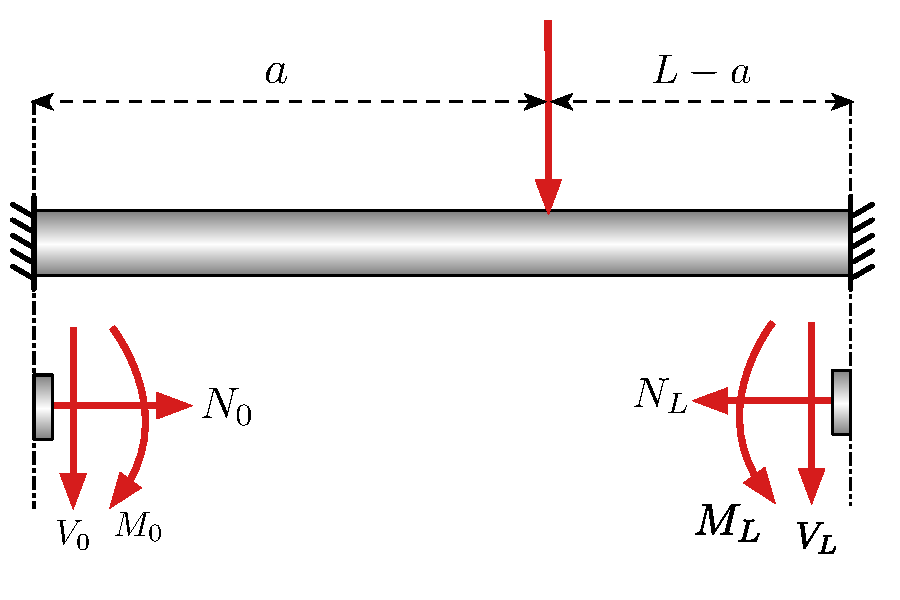
\includegraphics[width=0.5\columnwidth]{Figures/EqPointLoad}}
	\caption{Equivalent Nodal Load}
	\label{fig:EqPointLoad}
\end{figure}